\documentclass[9pt]{beamer}
\usetheme{Hannover} 

\usepackage{graphicx}
\usepackage{hyperref}
\usepackage{ifthen}
\usepackage{cancel}
\usepackage{empheq}
\usepackage[separate-uncertainty=true]{siunitx} 
\usepackage{subcaption}
\usepackage{setspace}

\usepackage[
    backend=biber,
    style=authoryear
]{biblatex}

\addbibresource{Slides/6.references.bib}


\newcommand{\degr}[0]{\text{$\text{}^\circ$}}


% Define your title page details

\title{Your Presentation Title}

\subtitle{}

\author{Fredrik Bergelv}

\date{\today}
\institute{
  Modelling of Large-Scale Circulation in Atmosphere and Ocean \\ (MO8004) 
}

% Is bibliography wanted (y/n)?
\newcommand{\IncludeBib}{n} 


\input{Other/Title.tex}

\begin{document}

\begin{frame}[plain]
  \titlepage
\end{frame}

\begin{frame}{Introduction}
  \section{Introduction}
  \begin{columns}[T] 
    \begin{column}{0.5\textwidth}

    Ocean circulation gyres are part of the atmospheric circulation.
    \begin{enumerate}
    \item Heating air at the equator $\rightarrow$ Hadley cells.
    \item Coriolis effect deflects the air movement $\rightarrow$ Trade winds and westerlies
    \item Enforce wind stress on the ocean surface $\rightarrow$ 90\degr  Ekman transport.
    \item Since $f$ increases with latitude, net southward Ekman transport in the North Atlantic. 
    \item Western boundary current needed to close the circulation.
    \end{enumerate} 

    \end{column}
    \begin{column}{0.5\textwidth} 
      \begin{figure}
    \centering
    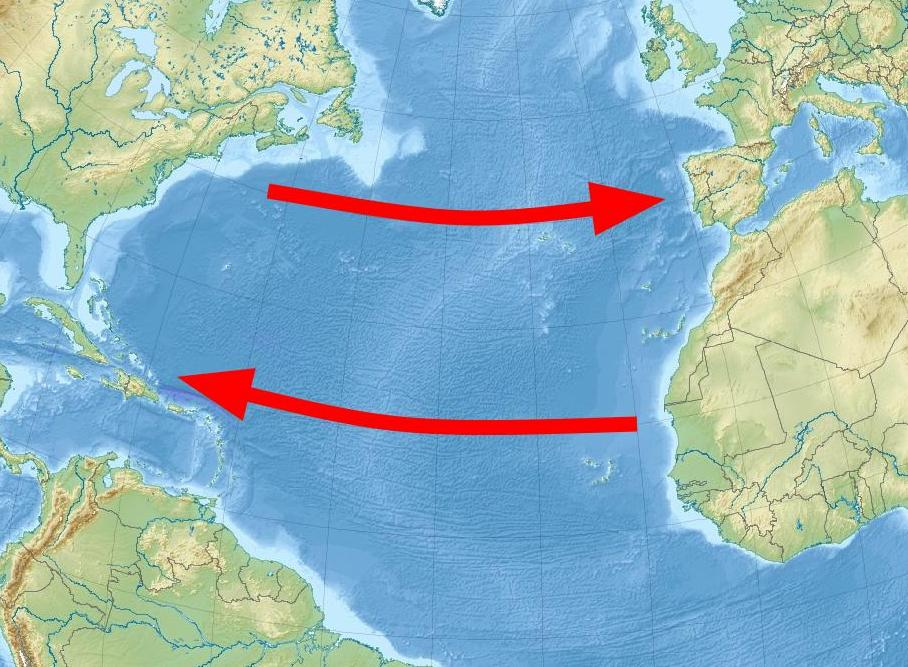
\includegraphics[width=\textwidth]{Figures/North_Atlantic.jpg}
    \caption{Wikimedia Commons, North Atlantic location map, accessed 2026}
  \end{figure}
    \end{column}
  \end{columns}
\end{frame}



\begin{frame}{Introduction, Sverdrup}
  \section{Theory}
  \subsection{Sverdrup}

  Harald Ulrik Sverdrup (1888-1957) formulated the net transport in the ocean interior as:

\begin{empheq}[box=\fbox]{equation}
  -\beta \frac{\partial \Psi}{\partial x} = \frac{1}{\rho}\nabla\times\vec{\tau}
\end{empheq}

which gives the Sverdrup solution:

\begin{equation*}
  \int_x^{x_\text{East}}\frac{\partial \Psi}{\partial x}\, dx = \int_x^{x_\text{East}} vH \, dx =
  \cancel{\Psi(x_\text{East},y)} - \Psi(x,y)
\end{equation*}
\begin{equation*}
  \implies\Psi(x,y) = -\frac{1}{\rho\beta}\int_x^{x_\text{East}} \left(\nabla\times\vec{\tau}\right) 
\end{equation*}
\end{frame}


\begin{frame}{Introduction, Munk}
  \subsection{Munk}

  Walter Heinrich Munk (1917-2019) extended the Sverdrup model by including meridional harmonic Newtonian viscosity (diffusion of momentum):
  \begin{empheq}[box=\fbox]{equation}
    A\nabla^4 \Psi -\beta \frac{\partial \Psi}{\partial x} = \frac{1}{\rho}\nabla\times\vec{\tau}
  \end{empheq}    

  which gives the Munk solution:
  \begin{align*}
    \Psi(x,y)=\Psi_{\text{Sverdrup}}(x,y)\Bigg(1-e^{-\frac{x-x_{\text{West}}}{2\delta_m}}\Bigg[ & \cos\!\left(\sqrt{3}\,\frac{x-x_{\text{West}}}{2\delta_m}\right)\\&+\frac{1}{\sqrt{3}}\sin\!\left(\sqrt{3}\,\frac{x-x_{\text{West}}}{2\delta_m}\right)\Bigg]\Bigg)
  \end{align*}

\begin{equation*}
  \text{ where } \delta_M\equiv\left(\frac{A}{\beta}\right)^{\tfrac{1}{3}}
\end{equation*}
\end{frame}



\begin{frame}{Method}
  \section{Method}

  Your content here.
\end{frame}



\begin{frame}{Result, The Sverdrup solution}
  \section{Result}
  \subsection{The Sverdrup solution}

  \begin{figure}[H]
    \centering    
    
\includegraphics[width=0.8\textwidth]{../../plots/no_drag_f_plane_streamfunction.png}
    \caption{Streamfunction for the no-drag $f$-plane configuration. The circulation remains symmetric with no $\beta$-effect and without western intensification.}
    \label{fig:f_plane_streamfunction}
\end{figure}

\end{frame}


\begin{frame}{Result, The Sverdrup solution}
  \section{Result}
  \subsection{The Sverdrup solution}

  \begin{figure}[H]
    \centering    
    
\includegraphics[height=0.3\textwidth]{../../plots/no_drag_f_plane_streamfunction.png}
    \caption{Streamfunction for the no-drag $f$-plane configuration. The circulation remains symmetric with no $\beta$-effect and without western intensification.}
    \label{fig:f_plane_streamfunction}
\end{figure}

\end{frame}




\begin{frame}{Discussion}
  \section{Discussion}
 
Both models show western boundary currents due to mass conservation, but only Munk theory shows a western boundary current. Why?:



\begin{columns}[T] 
    \begin{column}{0.6\textwidth}

    \begin{itemize}
        \item The Sverdrup theory is linear, only one B.C. $\Psi\left(x_\text{East}\right)=0$.
        \item The Munk theory is non-linear, four B.C.s: $\Psi\left(x_\text{East}\right)=\Psi\left(x_\text{West}\right)=v\left(x_\text{East}\right)=v\left(x_\text{West}\right)=0$.
        \item Frictional force is opposite sign to the motion itself, needed to balance Sverdrup flow. 
        \item The Munk viscosity creates a boundary layer where the frictional force can take care of mass conservation.
    \end{itemize}

    \end{column}
    \begin{column}{0.4\textwidth} 
        \vspace{1cm}
      \begin{empheq}{equation*}
            A\nabla^4 \Psi -\beta \frac{\partial \Psi}{\partial x} = \frac{1}{\rho}\nabla\times\vec{\tau}
       \end{empheq} 
    \end{column}
  \end{columns}

\end{frame}

\begin{frame}{Conclusion}
  \section{Conclusion}
 
Important conclusions:
\begin{itemize}
    \item Both numerical models showed western intensification, explained by Rossby wave propagation.
    \item Only Munk theory showed a western boundary current, explained by frictional layer, although both numerical models showed return flow close to the western boundary.
    \item A larger domain gave same interior meridional transport, which resulted in a stronger western boundary current.
\end{itemize}

\end{frame}


\begin{frame}
\frametitle{References}
  \nocite{*}
  \printbibliography
\end{frame}

\appendix
\begin{frame}{Extra figures}
\section{Appendix}
\begin{figure}[H]
    \centering    
    
\includegraphics[height=0.6\textwidth]{../../plots/munk_a_Nx.png}
    \caption{Streamfunction for the Laplace-viscous $\beta$-plane configuration. The red lines are the theoretical Munk solution. This figure has three times as high resolution (i.e. $\Delta x = \Delta y = 11.7\,\text{km}\implies \tfrac{\delta_M}{\Delta x}\approx\left[10, \, 15,\, 25\right]$) }
    \label{fig:munk_a_Nx}
\end{figure}
\end{frame}

\end{document}
